% -*- root: ../../main.tex -*
%!TEX root = ../../main.tex
% vim:textwidth=80 fo=cqt conceallevel=0

\subsection{Augmentation of parameters to standard \glsfmtshort{dfn} model}

\subsubsection*{Cell capacity and electrochemically active surface area}

The  \gls{p2d} implementation  of  the standard  \gls{dfn}  model lacks  certain
parameters that are vital to the  layer optimisation process. The cell's nominal
capacity is a fundamental quantity that gets  altered as the number of layers is
varied. However, it may be surprising  to discover that this parameter is absent
in present  research literature  discussing the  \gls{p2d} model.  The rationale
behind this glaring omission becomes clear  upon closer examination of the model
equations presented in  \cref{tbl:dfneqns}. These equations do not  operate on a
cell level, but  instead operate on a  normalised basis \ie{} only  one layer is
modelled on a  \emph{unit area} basis wherein the stimulus  driving the model is
the applied current  \emph{density} rather than the total  external current. The
layer  optimisation task  here faces  a unique  predicament of  adhering to  the
present modelling paradigm  to retain compatibility with  standard models whilst
still incorporating  the concept of cell's  capacity as a function  of number of
layers.

To  tackle the  aforementioned quandary,  it  is key  to realise  that the  core
parameter  that  varies with  the  number  of layers  in  a  pouch cell  is  the
\emph{electrochemically  active  cross-sectional surface  area}~$A_\text{cell}$.
Curiously, published  literature on  physics-based cell  modelling do  not place
rigorous emphasis on  this key parameter. Most often, to  this author's chagrin,
this  parameter is  simply  listed in  a  standard table  of  parameters and  is
typically  sourced from  a historic  parameter-set with  no further  explanation
provided.

For  a pouch  cell, the  overall electrochemically  active surface  area can  be
defined as
\begin{equation}\label{eq:overallarea}
    A_\text{cell} = n \times A_\text{elec}
\end{equation}
where $n$ is  the number of layers and $A_\text{elec}$  is the electrochemically
active surface area per layer.

\subsubsection*{Surface area per layer}\label{sec:surfareaperlayer}

A literature search reveals that akin  to cell capacity, there is no information
of  cross-sectional geometry  provided in  articles dealing  with the  \gls{p2d}
implementation of  the \gls{dfn} model. To  determine the surface area  per face
(per layer), the author proposes  a new methodology/process involving a sequence
of  steps, based  on  certain  assumptions and  literature  search. The  process
involves  selection of  a  real-world cell,  and ultimately  mapping  it to  the
surface area per  unit face. To the  best knowledge of the  author, this reverse
parametrisation process  (explained next), mapping  from a real-world cell  to a
\gls{p2d} parameter, is  a unique idea and  is claimed as a  contribution to the
art.

\begin{enumerate}[ label=\textbf{\arabic*}), leftmargin=0pt, itemindent=20pt, labelwidth=15pt, labelsep=5pt, listparindent=0.7cm, align=left]
    \item \hypertarget{refcellselection}{\textbf{Selection of a suitable reference capacity cell}}

        Although  this value  shall not  be used  in the  actual layer  optimisation
        procedure itself, this is a  crucial first-step towards obtaining a complete
        parameter set, in particular, to obtain the surface area per layer.

        The focus  of this chapter is  to provide ready-to-use solution  to industry
        extend  with the  aim of  improving  the current  state of  the art  through
        optimal layer configuration  of pouch cells. There is a  clear motivation to
        further increase  cell capacities so as  to maximize driving range,  as laid
        out in the beginning of this chapter (see \cref{sec:layeroptintro}).

        With  this  guiding  principle,  as  a starting  point  towards  choosing  a
        reference capacity cell,  a survey was performed to  identify the production
        \gls{bev}  with  the  highest  driving  range.  As  of  2018,~the  Chevrolet
        Bolt~\gls{bev} bears this distinction  with a range of \SI{383}{\kilo\meter}
        as rated  by the  United States Environmental  Protection Agency  (EPA). The
        specifications of  its battery pack is  listed in Liu~\etal~\cite{Liu2016a}.
        The  battery pack  of  this  vehicle consists  of  288~cells  arranged in  a
        96S-3P configuration, in  agreement with the configuration  discussed in the
        drivetrain  hierarchy  of  \cref{sec:packlevelhierarchy}.

        The    Chevrolet   Bolt    \gls{bev}   pack    has   an    energy   capacity
        of   \SI{60.0}{\kilo\watthour}    with   a    nominal   pack    voltage   of
        \SI{350}{\volt}~\cite{Liu2016a}.  However,  for   this  specific  task,  the
        \si{\amphour} capacity is required. This can be obtained as
        \begin{align}
            \text{\si{\amphour} capacity of Bolt cell} & = \frac{\text{Pack Energy } (\si{\watthour})}{\text{Nominal pack voltage (V)} \times {\text{Number of cells in parallel}}} \\
            {}                                         & = \frac{60000}{350 \times 3} \\
            {}                                         & = \SI{57.14}{\amphour}
        \end{align}

        \begin{itemize}[ leftmargin=10pt, itemindent=15pt, labelwidth=5pt, labelsep=5pt, listparindent=0.7cm, align=left]
            \item \textbf{DC bus voltage and revised cell capacity}

                Even  without  a  dc/dc  boost   converter,  robust  design  of  the
                powertrain during  brown-outs should  allow for  continued operation
                even   with   a  slightly   diminished   DC   bus  voltage   \approx
                \SIrange{4}{5}{\percent} lower than nominal~\cite{Maksimovic2012}.
                Considering a maximum permissible dip of \SI{4}{\percent} in the bus
                voltage \ie{} \SI{336}{\volt}, the cell's capacity may be refined as
                \begin{align}
                    \text{\si{\amphour} capacity of Bolt cell} & = \frac{\text{Pack Energy } (\si{\watthour})}{\text{Lowest pack voltage (V)} \times {\text{Number of cells in parallel}}} \\
                    {}                                         & = \frac{60000}{336 \times 3} \\
                    {}                                         & = \SI{59.52}{\amphour}
                \end{align}

                The reference cell's \si{\amphour} capacity is therefore rounded to
                \textbf{\SI{60}{\amphour}}\footnote{In the interest of maintaining consistency, this computed capacity is
                    retained for the cell used in
                    \crefrange{ch:spmanalysis}{ch:newelectrolytemodel} of this thesis. This also explains the use of \SI{60}{\ampere} for
                    the simulations demonstrating energy/power trade-off of
                    \cref{sec:energypowertradeoffdemo} since this current level corresponds to
                the 1C-rate of the cell.}.

            \item \hypertarget{celllowercutoff}{\textbf{Lower cutoff voltage for cells}}

                In  this  layer  optimisation  work, following  the  assumptions  of
                \cref{subsec:layeroptassumptions},  the  overall pack  configuration
                remains  unchanged  and  independent   of  layers  within  a  pouch.
                This  implies that  the undervoltage  threshold for  DC bus  voltage
                throughout  this   work  shall  remain  fixed   at  \SI{336}{\volt}.
                Therefore, with  96~series connected  cells in  a string,  the lower
                cut-off voltage for an  individual cell is \textbf{\SI{3.5}{\volt}}.
                This  value is  reported in  \cref{tbl:lcoSimParamslayeropt} and  is
                used as a termination condition  for all simulations as explained in
                \cref{sec:layeroptframework}.

        \end{itemize}

    \item \textbf{Computation of electrochemically overall active surface area for reference cell}

        For             the            cell             properties            in
        \crefrange{tbl:lcoSimParamsSPMp2d}{tbl:lcoSimParamslayeropt},        the
        majority                of                 parameters                are
        sourced           from          Subramanian~\etal~\cite{Subramanian2009}
        and                Northrop~\etal~\cite{Northrop2011}.                In
        Northrop~\etal~\cite{Northrop2011},  the   \emph{current  density}  that
        corresponds to  a 1C-rate discharge  of a  cell with this  parameter set
        is  reported to  be \approx  \SI{30}{\ampere\per\meter\squared}. In  the
        author's carefully  designed numerical simulations (very  slow discharge
        at C/500 from fully charged state until charge depletion), this value is
        refined to \SI{29.23}{\ampere\per\meter\squared}.

        The task of determining the electrochemically active overall surface
        area of the reference cell is now straightforward
        \begin{align}
            \text{Overall surface area of reference cell}, A_\text{refcell} &= \frac{\text{Cell capacity (\si{\amphour})}}{\text{1C-rate density (\si{\ampere\per\meter\squared})}} \\
                                                                            &= \frac{60}{29.23} \\
                                                                            &= \SI{2.053}{\meter\squared}
        \end{align}

        This  value  is  listed  in  \cref{tbl:lcoSimParamsSPMp2d}  for  use  in
        \crefrange{ch:spmanalysis}{ch:newelectrolytemodel},  but  is  \emph{not}
        used  in  this  layer  optimisation   work.  This  is  because,  as  the
        number  of  layers change,  the  overall  surface  area changes  as  per
        \cref{eq:overallarea}.

    \item \textbf{Setting the pouch height for the reference cell}

        Although the  official press release~\cite{GMBoltBatteryDims}  from the
        manufacturer  of this  \gls{bev} contains  data on  the cross-sectional
        geometry  of the  cell,  it does  not report  its  height. Hence,  this
        information  needs to  be assumed  by extrapolation  from an  alternate
        source wherein the conditions are similar and therefore, can be applied
        for this reference cell.

        The  review   article  by   Gr\"oger~\etal~\cite{Groger2015}  discusses
        various    states    of    the    art   in    energy    densities    of
        electrode   materials  used   in  various   lithium  ion   chemistries.
        At   the   time   of   its   publication,   the   areal   capacity   of
        cells  were  \approx  \SI{2.0}{\milli\amphour\per\centi\meter\squared}.
        These    authors   recommended    an   areal    capacity   target    of
        \SI{4.0}{\milli\amphour\per\centi\meter\squared} for  future automotive
        applications. This  publication also  considers the aspect  of stacking
        layers  into  pouches  of  certain  geometries.  In  particular,  table
        \romanletter{4}  of Gr\"oger~\etal~\cite{Groger2015}  considers a  pouch
        of  \SI{10}{\milli\meter} height,  for which  the aforementioned  areal
        capacities were calculated.

        In       the        case       of       the        reference       cell
        under       consideration,       the      areal       capacity       is
        \begin{equation}
            \text{Areal capacity of reference cell } = \frac{\SI{60000}{\milli\amphour}}{\SI{20527}{\centi\meter\squared}}  = \SI{2.92}{\milli\amphour\per\centi\meter\squared}
        \end{equation}
        which is close  to the desired value in automotive  applications as per
        the recommendations  in Gr\"oger~\etal. Considering that  the reference
        cell is  drawn from  the high energy  density Chevrolet  Bolt \gls{bev}
        cell,  a pouch  height of  \SI{10}{\milli\meter} is  justifiable for
        this task  and is  reported in \cref{tbl:lcoSimParamslayeropt}.  As per
        the assumptions discussed in \cref{subsec:layeroptassumptions}, this is
        held constant throughout the layer optimisation process.

    \item \hypertarget{stackthickness}{\textbf{Compute stack thickness of reference cell}}

        In a  pouch of given height,  the available space to  accommodate layers
        therein is restricted  by a number of factors. For  instance, the wiring
        from the  current collectors  to the tabs,  protective elements  such as
        fuses etc.\ consume space. For instance, the pouch material itself has a
        finite  thickness  and  hence  after  accounting  for  this,  the  stack
        thickness  available  for  layer  placement  is  lower  than  the  pouch
        thickness.
        \begin{align}
            \text{Stack thickness}, L_\text{stack} & = \text{Pouch height} - 2\times \text{pouch thickness} \\
            \text{Stack thickness}, L_\text{stack} & = H_\text{pouch} - 2 T_\text{pouch} \\
            L_\text{stack}(\si{\milli\meter})      & = 10.0 - 2\times(\num{160e-3}) \\
            L_\text{stack}                         & = \SI{9.68}{\milli\meter}
        \end{align}

        The value of stack thickness of  the reference cell is held constant for
        all layer choices used throughout the entire layer optimisation process.

    \item \textbf{Determination of number  of layers within  reference cell}

        The  next  step  is  to  determine  the  number  of  layers  within  the
        reference pouch  cell~$n_\text{refcell}$.

        The thickness of a complete electrochemical sandwich multiplied by the
        number of layers yields the total stack height
        \begin{equation}\label{eq:stackheightrefcell}
            n_\text{refcell}\, (l_\text{Al} + l_\text{pos} + l_\text{sep} + l_\text{neg} + l_\text{Cu}) = L_\text{stack}
        \end{equation}

        The product of  layers and the thickness of  an electrochemical sandwich
        cannot exceed the  overall stack height. This implies  that the equality
        in \cref{eq:stackheightrefcell} is  to be changed to  an inequality with
        the upper  bound of the  computation on the  \gls{lhs} set to  the stack
        height.
        \begin{align}
            n_\text{refcell}\, (l_\text{Al} + l_\text{pos} + l_\text{sep} + l_\text{neg} + l_\text{Cu}) & \le L_\text{stack} \\
            n_\text{refcell}                                                                            & \le \frac{L_\text{stack}}{l_\text{Al} + l_\text{pos} + l_\text{sep} + l_\text{neg} + l_\text{Cu}}\label{eq:stackheightrefcellmod}
        \end{align}

        Since fractional layers do not have  any physical meaning, the number of
        layers that  can be  accommodated within  any pouch  must be  an integer
        quantity. Therefore,  $n_\text{refcell}$ is  computed as the  `floor' of
        the quantity in the \gls{rhs} of \cref{eq:stackheightrefcellmod}
        \begin{align}
            n_\text{refcell} &= \floor*{\frac{L_\text{stack}}{l_\text{Al} + l_\text{pos} + l_\text{sep} + l_\text{neg} + l_\text{Cu}}} \\
            {} &= \floor*{\frac{9.68}{(15 +  72 + 25 + 88 + 10) \times 10^{-3}}} \\
            n_\text{refcell} &= 46
        \end{align}

        The reference cell is thus deemed to consist of 46~layers.

    \item \textbf{Computation of surface area per layer}

        Substituting  the values  of  $n_\text{refcell}$ and  $A_\text{refcell}$
        into  \cref{eq:overallarea}, the  electrochemically active  surface area
        per layer is obtained as
        \begin{align}
            A_\text{elec} & = \frac{A_\text{refcell}}{n_\text{refcell}} \\
            {}            & = \frac{\SI{2.053}{\meter\squared}}{46}     \\
            {}            & = \SI{44.63}{\milli\meter\squared}
        \end{align}

        The   surface   area   per   layer    thus   computed   is   listed   in
        \cref{tbl:lcoSimParamslayeropt} and  is held constant  throughout across
        all  layer choices  tried during  the layer  optimisation process.  This
        assumption  is  immediately  justifiable   from  a  physical  viewpoint,
        since  the process  of assembling  layers is  along the  axial thickness
        direction (aligned with  pouch height) and is independent  of the planar
        (cross-sectional) direction.

\end{enumerate}

\subsection{Modification of standard \glsfmtshort{dfn} model to handle power inputs}\label{sec:innatepowerinput}

As   discussed  in   \cref{sec:packlevelhierarchy},   assuming  identical   cell
conditions during operation necessitates that the external stimulus to the cells
is an applied power  value. The cell's terminal voltage as  well as current draw
can  be viewed  as a  natural response  to this  power input.  To simulate  this
condition  for  achieving  a  model-based optimal  layer  design,  the  standard
\gls{dfn} model ---  which conventionally handles current stimuli ---  has to be
suitably modified to accept power inputs.

Plett~\cite{Plett2016}  suggests  a methodology  for  applying  power inputs  to
equivalent  circuit models  simulated  at  a fixed  sample  rate. This  involves
converting the input  power~$P_k$ to a current~$I_k$ using  an equivalent series
resistance~$R_0$. The value  of $R_0$ is updated at every  time index~$k$ as per
\cref{eq:PlettPower}.  $v_k$ is  the  cell's terminal  voltage  at present  time
sample $k$, which has been evolved from  the applied current up to and including
the previous time step $(k-1)$.
\begin{equation}\label{eq:PlettPower}
    I_k = \frac{v_k - \sqrt{v^\text{2}_k - 4R_0P_{k}}}{2R_0}
\end{equation}

There  are  two disadvantages  in  using  Plett's  simplified approach  for  the
proposed layer optimisation study. Firstly, this necessitates the quantification
of the electrical resistance of a \gls{pbm}. Such an idea is at loggerheads with
the fundamental philosophy  of \glspl{pbm} which strive to  represent a detailed
picture  of  underlying  phenomena,  as opposed  to  the  system-level  terminal
behavioural characterisation  facilitated by the \glspl{ecm}.  Translating power
to current  in this manner also  necessitates a two-pass conversion  between the
physical domain and the electrical domain  --- a process likely to significantly
degrade the modelling fidelity. Since the  results from application of the model
shall inform the number  of layers to be used in a  real-world cell design, such
loss of fidelity  is unacceptable. Secondly, the constraint of  using fixed time
interval updates implies that a  high-speed adaptive time-stepping solver cannot
be  used for  handling this  power  input condition.  This shall  slow down  the
simulation speed considerably since the search space of layer combinations to be
considered is  fairly large.  Furthermore, the simulations  have to  be repeated
over  multiple combinations  of  initial and  ambient  temperatures which  shall
render the model-based design approach to  be too slow and offset its advantages
over a conventional prototype-based design.

Dees~\etal~\cite{Dees2002}  identified the  requirement  of  having a  \gls{p2d}
model that  can run on applied  power. However, in the  aforementioned work, the
relevant  equations for  reformulation  of solid-phase  boundary conditions  are
not  presented. This  thesis  author  therefore feels  compelled  to provide  an
independent derivation  of reformulating  the \gls{p2d}  model to  facilitate an
innate power  input capability.  Since the  equations are  derived for  a single
layer, the  power \emph{density}, obtained by  scaling the applied power  by the
overall  active cross-sectional  area~$A_\text{cell}$,  is used  as the  driving
input.

In  the  \gls{p2d}  model,  charge  conservation in  solid  phase  is  given  by
\cref{eq:solidchargeconserve},  which is  revisited  below.  The subsequent  two
equations pertain to the corresponding  boundary conditions. In these equations,
the current density~$i$ represents the applied input.
\begin{align}
    \frac{\partial}{\partial x} \left(\sigma_{\text{eff}} \frac{\partial \phi_\text{s}(x,t)}{\partial x} \right) &= a_\text{s} F j(x,t) \tag{\cref{eq:solidchargeconserve} revisited}\\
    \sigma_{\text{eff}} \frac{\partial \phi_\text{s}(x,t)}{\partial x} \bigg|_{\substack{x_\text{pos/Alcc}\\x_\text{neg/Cucc}}} &= -i\label{eq:solidchargeconservecurrBC}\\
    \sigma_{\text{eff}} \frac{\partial \phi_\text{s}(x,t)}{\partial x} \bigg|_{\substack{x_\text{pos/sep}\\x_\text{neg/sep}}} &= 0
\end{align}

Now,  \cref{eq:undiscretisedPhiSpowerBC}  replaces  the boundary  condition  in
\cref{eq:solidchargeconservecurrBC}  to use  the  applied  power density~$p$  to
drive the model.

\begin{equation}\label{eq:undiscretisedPhiSpowerBC}
    \sigma_{\text{eff}_\text{neg}} \left( \phi_\text{s}(x,t) \frac{\partial
            \phi_\text{s}(x,t)}{\partial
            x}\right)\Bigg\rvert_{\mathrlap{x=x_\text{neg/Cucc}}}  -
        \sigma_{\text{eff}_\text{pos}} \left( \phi_\text{s}(x,t) \frac{\partial \phi_\text{s}(x,t)}{\partial x} \right)\Bigg\rvert_{\mathrlap{x=x_\text{pos/Alcc}}} = p
\end{equation}

\Crefrange{eq:ctspowerconstraint}{eq:cellpositivity}  represent the  constraints
pertaining to physical laws and are to be satisfied.
\begin{align}
	vi  - p & = 0 \label{eq:ctspowerconstraint} \\
	v       & > 0 \label{eq:cellpositivity}
\end{align}
\Cref{eq:ctspowerconstraint}   denotes  that   the  product   of  the   terminal
voltage   and   computed   current    density   shall   equal   the   externally
applied  power  density,  whereas   \cref{eq:cellpositivity}  implies  that  the
cell's  terminal   voltage  shall  always  remain   positive  during  operation.
\Crefrange{eq:undiscretisedPhiSpowerBC}{eq:cellpositivity} are  then discretised
for numerical implementation.

\Cref{fig:1d_fv_mesh}  describes  a  schematic  overview  of  a  one-dimensional
cell-centred  \gls{fv}  discretisation scheme.  Here,  evenly  spaced nodes  are
considered to form  the support mesh along the through-thickness  dimension of a
layer. Vertical  lines denote the  edges of  control volumes whereas  the filled
circles depict  computational nodes where the  variables from \cref{tbl:dfneqns}
pertaining to the axial direction are solved.

\begin{figure}[!htbp]
    \centering
    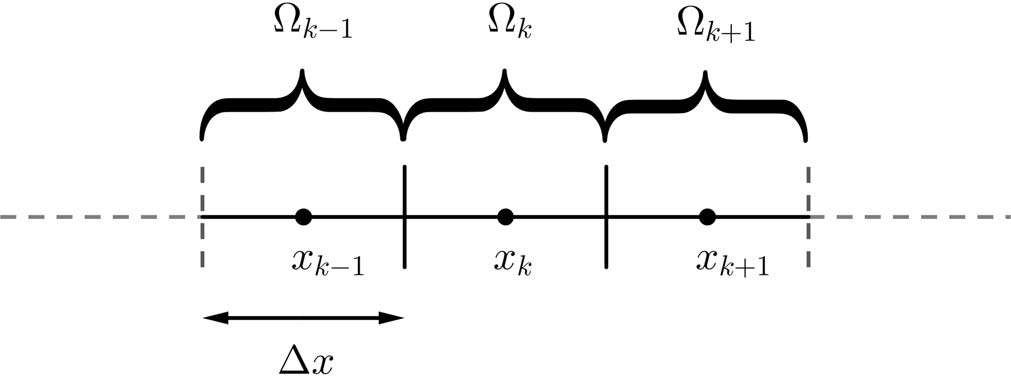
\includegraphics{fv_disc.jpg}
    \caption[Illustration of a standard cell-centred \gls{fv} discretisation
    scheme]{Simplified illustration of a standard cell-centred \gls{fv}
    discretisation scheme. Image reproduced from
Torchio~\etal~\cite{Torchio2016}.}
    \label{fig:1d_fv_mesh}
\end{figure}

\Cref{eq:discretisedPhiS}      represents       the      weak       form      of
\cref{eq:solidchargeconserve} used on the \gls{fv}  mesh in each control volume,
wherein subscripts~$k$ and  $k\pm\frac{1}{2}$ denote the $k$\textsuperscript{th}
\gls{fv} node and its associated left and right edges respectively.
\begin{equation} \label{eq:discretisedPhiS}
    \sigma_{\text{eff}} \frac{\partial \phi_\text{s}(x,t)}{\partial x}\Bigg|_{x_{k-\frac{1}{2}}}^{x_{k+\frac{1}{2}}} = a_\text{s} F j_k(t) \Delta x
\end{equation}

At this juncture, a simplifying approximation for the solid-phase potentials can
be considered. In the standard \gls{fv} scheme, the solution values at the faces
(edges of  control volumes) is  obtained by  interpolating from the  two nearest
\gls{fv} node values.  At the two extrema of the  computational domain, a linear
extrapolation from  the first and last  nodes can be considered.  Accounting for
this increases the accuracy of  computations thereby providing good estimates of
solid  potentials at  the  interfaces. However,  this comes  at  the penalty  of
producing  a  mathematically complex  set  of  boundary conditions.  When  using
high  node  densities  in  the  negative and  positive  electrode  regions  (see
\cref{tbl:lcoSimParamslayeropt}),  for the  two outermost  control volumes,  the
values  of $\frac{\Delta  x}{2}$ becomes  small.  With a  reasonably small  mesh
interval, the  potentials at  the cell  centres can be  considered to  be nearly
equal  to  that  at  their  corresponding  current  collector  interfaces.  This
assumption helps to keep the resulting mathematical expressions tractable.

Applying    \cref{eq:discretisedPhiS}    to    the    first    control    volume
(0\textsuperscript{th} node) in  the positive electrode and to  the last control
volume (n\textsuperscript{th} node) in the negative electrode,
\begin{align}
	\frac{-\sigma_{\text{eff}_\text{pos}} \phi_{\text{s}_0}}{\Delta x_\text{pos}} + \frac{\sigma_{\text{eff}_\text{pos}} \phi_{\text{s}_1}}{\Delta x_\text{pos}} + i &= a_{\text{s}_\text{pos}} F j_0 \Delta x_\text{pos}\label{eq:PhiSappliedBCpos}\\
	\frac{-\sigma_{\text{eff}_\text{neg}} \phi_{\text{s}_n}}{\Delta x_\text{neg}} + \frac{\sigma_{\text{eff}_\text{neg}} \phi_{\text{s}_{n-1}}}{\Delta x_\text{neg}} - i &= a_{\text{s}_\text{neg}} F j_n \Delta x_\text{neg}\label{eq:PhiSappliedBCneg}
\end{align}

Subtracting the equations  resulting from multiplying \cref{eq:PhiSappliedBCpos}
with $\phi_{\text{s}_0}$ and \cref{eq:PhiSappliedBCneg} by $\phi_{\text{s}_n}$
\begin{multline} \label{eq:pinputBCcomplete}
    \frac{-\sigma_{\text{eff}_\text{pos}} \phi^2_{\text{s}_0}}{\Delta x_\text{pos}} -
    \frac{\sigma_{\text{eff}_\text{neg}} \phi^2_{\text{s}_n}}{\Delta x_\text{neg}} +
    \frac{\sigma_{\text{eff}_\text{pos}} \phi_{\text{s}_0} \phi_{\text{s}_1}}{\Delta x_\text{pos}} +
    \frac{\sigma_{\text{eff}_\text{neg}} \phi_{\text{s}_n} \phi_{\text{s}_{n-1}}}{\Delta x_\text{neg}} \\+ p -
    a_{\text{s}_\text{pos}} F j_0 x_\text{pos} \phi_{\text{s}_0} - a_{\text{s}_\text{neg}} F j_n x_\text{neg}
    \phi_{\text{s}_n} = 0
\end{multline}

\fxnote{figure showing power input}

Two solutions  exist for  the quadratic equation  in \cref{eq:pinputBCcomplete}.
However, solid  phase potential being a  physical quantity of the  cell needs to
have a unique solution. Therefore, in order to achieve numerical convergence, an
additional positivity constraint is imposed.
\begin{equation}\label{eq:discpositivity}
	\phi_{\text{s}_0} - \phi_{\text{s}_n} > 0
\end{equation}

Finally  since the  input to  the model  is the  applied power  density~$p$, the
current  density  within  each  layer~$i$  needs  to  be  solved  for.  This  is
facilitated by  employing the discretised form  of \cref{eq:ctspowerconstraint}.
Furthermore, since  this equation  is mathematically simple,  the aforementioned
assumption of  using node values  at current  collector interfaces is  no longer
required.  Applying  a  linear  extrapolation  scheme,  the  algebraic  residual
equation is obtained as
\begin{equation}\label{eq:currdensityresidual}
    0 = i - \frac{p}{1.5 \phi_{\mathrm{s}_0} - 0.5 \phi_{\mathrm{s}_1} + 0.5 \phi_{\mathrm{s}_{n-1}} - 1.5 \phi_{\mathrm{s}_{n-1}}}
\end{equation}
The    computer    code   used    (LIONSIMBA~v2.0,    to    be   discussed    in
\cref{sec:resultslayeropt}) employs the \gls{dae} solver IDA~\cref{sundials2005}
to handle such algebraic constraints.

\Crefrange{eq:pinputBCcomplete}{eq:currdensityresidual} therefore represents the
reformulated  boundary condition  and associated  algebraic constraints  for the
solid  phase potential  \gls{pde} that  can be  applied to  either electrode  to
facilitate the use of an input power density to the \gls{p2d} model.

\subsection{Hybrid spectral-\glsfmtshort{fv} scheme}\label{sec:hybridfv-spectral}

Fast  and  accurate  estimation  of   the  solid  phase  lithium  concentration,
particularly  its   value  at   the  surface  of   electrode  particles   is  an
inherent  requirement   of  the   layer  optimisation  procedure   presented  in
\cref{sec:layeroptframework}.   The  high   power  densities   to  be   handled,
particularly  at  low   layer  counts  necessitate  this   requirement.  It  has
been   acknowledged  that   solid-phase  concentration   calculations  employing
polynomial    approximations   lack    fidelity    at   high    charge/discharge
rates~\cite{Santhanagopalan2006}.  Hence,  a  conventional  full-order  solution
based on Fick's law of diffusion is required for this layer optimisation task.

With full-order  solid phase  diffusion dynamics,  applying the  \gls{fv} scheme
(that has been  employed in LIONSIMBA~v1.0x to  discretise all through-thickness
\gls{pde}s of the \gls{p2d} model) results  in a very large system of equations.
This is due to the requirement of using a high radial node density per spherical
particle for improved accuracy. Consequently, the computational cost is high and
simulation  runtime  becomes prohibitive  when  exploring  the search  space  of
all  possible  layer configurations.  Moreover,  with  a cell-centered  \gls{fv}
discretisation,  it is  non-trivial to  directly apply  the ionic  flux boundary
condition at the particle surface, since it involves extrapolation from at least
two other nodes within the particle. While such extrapolations are acceptable in
the axial  dimension --- particularly  with high node densities  providing small
values of $\frac{\Delta x}{2}$ --- they are undesirable in the radial dimension.
This  is because  cell's  open  circuit and  terminal  voltages strongly  depend
on  the  concentration  at  the  particle  surface.  Spectral  methods  offer  a
combination  of high  accuracy and  speed while  permitting the  use of  a lower
number  of radial  discretisation nodes.  To implement  a spectral  scheme on  a
non-periodic  domain,  a  Chebyshev discretisation~\cite{Trefethen2000}  may  be
applied.  Bizeray~\etal{}~\cite{Bizeray2015} discretised  all  of the  \gls{p2d}
model  equations using  this approach.  However, this  entails a  bi-directional
mapping of all  variables between the physical and  Chebyshev domains, incurring
computational overhead.

In this chapter, a hybrid formulation of the \gls{p2d} model is proposed wherein
a standard \gls{fv} scheme  in the axial dimension and a  spectral scheme in the
radial domain  are used.  Exploiting this  natural separation  of the  axial and
radial domains enables to ---
\begin{enumerate*}[label=\roman*)]
    \item retain  the   ability  to  easily   couple  the   molar  flux  density   at  the particle  surface  through  reformulation  of the  boundary  conditions  of  the solid  diffusion \gls{pde},  and
    \item solve  for  solid-phase  lithium  concentration  in  the  Chebyshev  domain  and locally transform  to physical  domain, without requiring  system-wide Chebyshev reformulations.
\end{enumerate*}
Although the proposed implementation does  not \emph{globally} employ a spectral
scheme, the  combined beneficial  effects of  radial-domain spectral  scheme and
automatic differentiation of system equations using CasADi~\cite{Andersson2013b}
facilitates rapid simulation, enabling  layer optimisation on short time-scales.
\Crefrange{eq:defineChebNodes}{eq:solidDiffEqChebDomain}   detail  the   steps
leading to  the reformulated solid  phase diffusion and its  associated boundary
condition in the Chebyshev domain.

The $N_\text{r}$~Chebyshev collocation nodes, defined on a 1D mesh in the radial
direction, are given by \cref{eq:defineChebNodes}~\cite{Trefethen2000}.
\begin{equation}\label{eq:defineChebNodes}
    \widetilde{r} = \cos\left(\frac{i\pi}{N_\text{r}}\right), \qquad i = 0, 1, \dots N_\text{r} \quad \widetilde{r} \in [-1, 1]
\end{equation}

Assuming  constant diffusivity,  and expanding  the derivative  in the  standard
form of  the Fickian  spherical diffusion equation  (see \cref{eq:dfnsoliddiff})
for  each particle,  we  obtain  \cref{eq:quotientappliedpde}, presented  along
with  its   Neumann  boundary   conditions \cref{eq:quotientappliedpdeBCcentre}
and \cref{eq:quotientappliedpdeBCsurface}.  $j$~is   the  molar   flux  density
(\si{mol.m^{-2}.s^{-1}}) and $R_\text{p}$ is the particle radius (\si{m}).
\begin{subequations}\label{eq:quotientappliedpde}
    \begin{align}
        \frac{\partial c_\text{s}}{\partial t} &= D^\text{eff}_\text{s} \left( \frac{\partial}{\partial r} \frac{\partial c_\text{s}}{\partial r} + \frac{\partial^2 c_\text{s}}{\partial r^2} \right) \qquad r \in [0, R_\text{p}]\tag{\ref*{eq:quotientappliedpde}}\\
        \diffp{c_\text{s}}{r}{\mathrlap{r = 0}} &= 0\label{eq:quotientappliedpdeBCcentre}\\
        D^\text{eff}_\text{s}\diffp{c_\text{s}}{r}{\mathrlap{r = R_\text{p}}} &= -j\label{eq:quotientappliedpdeBCsurface}
    \end{align}
\end{subequations}

Mapping $r \in [0,R_\text{p}] \mapsto \widetilde{r} \in [-1, 1]$,
\begin{equation}\label{mappingChebDomain}
    r = \frac{R_\text{p}}{2}(\widetilde{r} + 1)
\end{equation}

Applying \cref{mappingChebDomain} to
\crefrange{eq:quotientappliedpde}{eq:quotientappliedpdeBCsurface} whilst
retaining $c_\text{s}$ in the physical space yields
\crefrange{eq:solidDiffEqChebDomain}{eq:solidDiffEqChebDomainBCsurface}.

\begin{subequations}\label{eq:solidDiffEqChebDomain}
    \begin{align}
	    \frac{\partial c_\text{s}}{\partial t}                         & = 4 \frac{D^\text{eff}_\text{s}}{R_\text{p}^2} \left( \frac{2}{\widetilde{r} + 1} \frac{\partial c_\text{s}}{\partial \widetilde{r}} + \frac{\partial^2 c_\text{s}}{\partial {\widetilde{r}}^2} \right)\tag{\ref*{eq:solidDiffEqChebDomain}} \\
        \diffp{c_\text{s}}{\widetilde{r}}{\mathrlap{\widetilde{r}=-1}} & = 0\label{eq:solidDiffEqChebDomainBCcentre}                                                                                                                                                                                                                \\
        2 \frac{D^\text{eff}_\text{s}}{R_\text{p}} \diffp{c_\text{s}}{\widetilde{r}}{\mathrlap{\widetilde{r}=1}} & = -j\label{eq:solidDiffEqChebDomainBCsurface}
    \end{align}
\end{subequations}

During  the iterative  solution process,  the spatial  gradients of  solid phase
lithium concentration  in \cref{eq:solidDiffEqChebDomain}  in this case  are not
computed through  an explicit  differentiation procedure  as usual,  but instead
evaluated by pre-multiplying  the concentration values at  the collocation nodes
by a Chebyshev differentiation matrix. This particular aspect is responsible for
the inherent reduction of simulation  runtime achieved by introducing a spectral
method. In the updated version  of LIONSIMBA~v2.0 (created specifically for this
layer  optimisation work),  differentiation matrices  of suitable  dimensions as
well as the Chebyshev collocation nodes  are generated using the MATLAB function
\texttt{cheb.m}~\cite{Trefethen2000}.

\fxnote{Layerphoto showing face areas and anode/cathode overhang?}

